\section{Мат. аппарат и определения}
% \begin{definition}
%     \textit{Гауссова поверхность} -- это замкнутая поверхность в трехмерном пространстве, через которую рассчитывается поток векторного поля.
% \end{definition}

% \begin{definition}
%     \textit{Замкнутая поверхность} -- компактная поверхность без края (границы).
% \end{definition}

\begin{definition}
    Векторное поле -- это отображение из $S \subset \mathbb{R}^n \mapsto \mathbb{R}^n$, сопоставляющее каждой точке вектор. В нашем случае из $S \subset \mathbb{R}^3 \mapsto \mathbb{R}^3$.
\end{definition}

\begin{definition}
    Пусть заданы $\overline{G} \subset \mathbb{R}^2$ замкнутая ограниценная область с границей $\partial G$ -- простым кусочно-гладким контуром. $\Sigma$ -- простая гладкая поверхность, заднная отображеним $x: \overline{G} \mapsto \mathbb{R}^3$ и ориентированная одним из двух непрерывных полей единичных нормалей $$n(x) = \pm \frac{[x'_{t^1}, x'_{t^2}]}{\Vert[x'_{t^1}, x'_{t^2}] \Vert_2}:\ \Sigma\ \backslash\ \partial \Sigma \mapsto \mathbb{R}^3$$ 
    Далее пусть задано векторное поле $F = (F^1, F^2, F^3): \ \Sigma\ \backslash\ \partial \Sigma \mapsto \mathbb{R}^3$. Тогда потоком векторного поля $F$ через ориентированную поверхность $\Sigma$ называется величина $$\iint_\Sigma F d\sigma = \pm \iint_G <F, \Vert[x'_{t^1}, x'_{t^2}] \Vert_2>dt$$
    где $<a, b>$ -- скалярное произведение.
\end{definition}

\begin{remark}
    Чтобы лучше понять, что понятие потока векторного поля, посмотрите физическую интерпритацию этого понятия в законе Гаусса.
\end{remark}

\begin{definition}
    Набор слуайных величин $\xi = (\xi_1,..., \xi_n)$ имеет \textit{многомерное нормальное распределение}, если:
    \begin{enumerate}
        \item $\exists\ a = (a_1,..., a_n)$, где $a_i \in \mathbb{R}$. Этоот вектор называется \textit{вектором средних многомерных нормального распределения}. 
        \item $\exists\ C = (c_{ij})$ -- матрица, в которой $c_{ij} \in \mathbb{R}$
        \item $\exists$ набор независимых стандартных нормальный случайных величин $\eta = (\eta_1,..., \eta_n)$ (то есть $\eta_i \sim  \mathcal{N}(0,1)$) для которых выполнено 
        $$\begin{cases}
            \xi_1 = a_1 + c_{11}\eta_1 +...+ c_{1n}\eta_n\\
            \dots\\
            \xi_n = a_n + c_{n1}\eta_1 +...+ c_{nn}\eta_n
        \end{cases} \Longleftrightarrow \xi = a + C \eta$$
    \end{enumerate}
    
\end{definition}

\begin{definition}
    \textit{Матрица ковариации} $B = (b_{ij})$ называется матрица, такая что $(b_{ij}) = cov(\xi_i, \xi_j)$ 
\end{definition}

\begin{remark}
    Матрицы связаны следующим образом: $B = B\cdot B^T$ 
\end{remark}

\section{Описание Gaussian Splatting}
\begin{definition}
    GS -- это гибридный метод объемной визуализации.\\
    Сцена для GS - это массив примитовов. Примитивы обладают мледующими параметрами:
    \begin{enumerate}
        \item $(x, y, z)$ -- координаты положения центра масс Гауссиана в пространстве.
        \item Для многомерного нормального (гауссовского) распределения нужна ковариационная матрица размерности $3\times3$, которая показывает, насколько вытянут или сплюснут эллипсоид.
        \item Альфа-канал (дополнительный канал, который хранит информацию о прозрачности, позволяя создавать частичную или полную прозрачность элементов)
        \item RGB
    \end{enumerate}
    
\end{definition}


\section{Описание 3D-GS}

3D-GS -- это фреймворк для создания сцен динамического вождения. Он моделирует статическую сцену с помощью множества трехмерных
гауссов. Для сложных сцен с движущимися объектами сначала последовательно моделируем статический фон всей сцены с помощью дополнительных статических 3D-гауссиан. Затем мы используем составной динамический гауссовский граф для обработки множества движущихся объектов, индивидуально реконструируя каждый объект и восстанавливая их точное положение
и взаимосвязи между перекрытиями в пределах сцены. Далее мы
используем лидарный анализатор для гауссовского разбрызгивания для реконструкции сцены с большей детализацией и сохранением панорамной
целостности.\\
\href{https://github.com/VDIGPKU/DrivingGaussian}{Репо с фреймом}\\
\href{https://habr.com/ru/articles/228525/}{Классическая реализация SfM}\\
\href{https://huggingface.co/blog/gaussian-splatting}{Введение в 3D-GS}\\
\href{https://github.com/graphdeco-inria/diff-gaussian-rasterization}{Дифференциальная гауссовская растеризация}

\section{Incremental Static 3D Gaussians}
\textbf{Проблемы:}
\begin{itemize}
    \item По мере движения эго-машины статический фон часто претерпевает временные сдвиги и изменения.
    \item Из-за принципа перспективы (проблема точки схода) предварительная интеграция отдаленных уличных сцен с разных временных шагов, находящихся далеко от текущей камеры, может привести к путанице масштаба, неприятным артефактам и размытости.
\end{itemize}
\textbf{Решение:}
Улучшаем 3D-GS, вводя инкрементальные статические 3D Гауссианы, используя изменения перспективы, вызванные движением машины, и временные отношения между соседними кадрами.
\begin{enumerate}
    \item Делим статическую сцену на N бинов на основе диапазона глубины, предоставленного LiDAR. Бины располагаются в хронологическом порядке, обозначаемом как ${b_i}^N$, где каждый бин содержит изображения с одной или нескольких временных точек.
    \item Для сцены внутри первого бина мы инициализируем модель Гауссиана, используя LiDAR (аналогично применимый к точкам SfM):
    $$p_{b_0}(l|\mu, \Sigma) = e^{-\frac{1}{2}(l-\mu)^T \Sigma^{-1} (l-\mu)}$$
    где $l \in \mathbb{R}^3$ --  позиция LIDAR; $\mu$ -— среднее значение точек LiDAR; $\Sigma \in Mat_{3\times 3}(\mathbb{R} )$  — анизотропная матрица ковариации; и T — оператор транспонирования.\\
    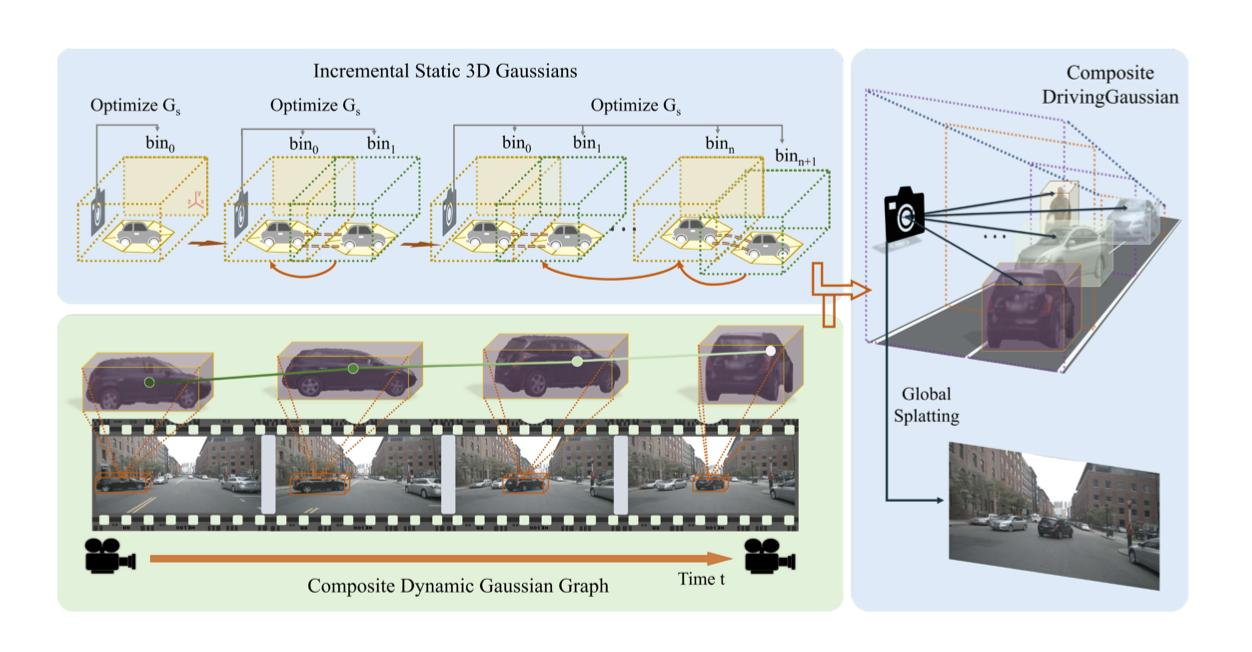
\includegraphics[scale = 0.35]{../pictures/pic3.JPG}
    \item Для следующих бинов используем Гауссианы из предыдущего бина в качестве прежних позиций и выравниваем смежные бины на основе их перекрывающихся регионов. 3D-центр для каждого бина может быть определен как:
    $$\hat{P}_{b+1}(G_s) = P_b(G_s) \cup (x_{b+1}, y_{b+1}, z_{b+1})$$
    где $\hat{P}$ -- это коллекция 3D-центров для Гауссиан $G_s$ всех в данный момент видимых регионов, $(x_{b+1}, y_{b+1}, z_{b+1})$ -- координаты Гауссиан внутри региона b+1.
    \item Итеративно мы добавляем сцены из последующих бинов в ранее построенные Гауссианы с использованием нескольких окружающих кадров. Инкрементальная статическая модель Гауссиан $G_s$ может быть определена как:
    $$\hat{C}(G_s) = \sum_{b=1}^{N} \Gamma_b \alpha_b C_b, \quad \Gamma_b = \prod_{i=1}^{b-1} (1 - \alpha_b)$$
    где $C$ -- цвет, соответствующий каждому одиночному Гауссиану при определенном ракурсе, $\alpha$ — непрозрачность, а $\Gamma$ — накопленная пропускаемость сцены в соответствии с $\alpha$  по всем бинам. Во время этого процесса перекрывающиеся регионы между окружающими изображениями с нескольких камер используются для совместного выравнивания моделей Гауссиан.
    \item Обратите внимание, что во время инкрементального построения статических моделей Гауссиан могут возникнуть различия в сэмплировании одной и той же сцены между передней и задней камерами. Чтобы устранить это, мы применяем взвешенное усреднение для точной реконструкции цветов сцены, насколько это возможно, во время 3D-проекции Гауссиан:
    $$\hat{C} = s(G_s) \sum w(\hat{C}(G_s) | R, T)$$
    где $\hat{C}$ — оптимизированный цвет пикселя, s -- дифференциальное сплаттинг, $w$ — вес для разных ракурсов, $[R, T]$ — матрица вида для выравнивания видов с нескольких камер.
\end{enumerate}

\section{Приоритет LiDAR с учетом окружающих видов}
\textbf{Проблема:} 3D-GS пытается инициализировать Гауссианы через SfM. Однако неограниченные городские сцены для автономного вождения содержат множество многоуровневых фонов и передних планов. Тем не менее, они видны только через чрезвычайно разреженные ракурсы, что приводит к трудоемкому и неполному восстановлению геометрических структур.\\
\textbf{Решение:} 
Для лучшей инициализации Гауссиан мы вводим приоритет LiDAR для 3D Гауссиан, чтобы получить более точные геометрии и поддерживать согласованность между несколькими камерами в регистрации окружающих видов. 
\begin{enumerate}
    \item Пусть $t \in T$ -- временной шаг; $\{I_t^i\}_{i = 1}^N$ -- набор изображений с нескольких камер, собранных с движущейся платформы; $L_t$ -- многокадровые сканирования LiDAR.
    \item Хотим: минимизировать ошибки регистрации между камерами, используя данные LiDAR-изображений, и получить точные позиции точек и геометрические приоритеты.
    \item Сначала мы объединяем несколько кадров сканирований LiDAR, чтобы получить полное облако точек сцены, обозначаемое как $L$. Мы следуем Colmap и извлекаем признаки изображения $X = x_q^p$ из каждого изображения индивидуально.
    \item Затем мы проецируем точки LiDAR на окружающие изображения. Для каждой точки LiDAR $l$ мы преобразуем ее координаты в систему координат камеры и сопоставляем ее с 2D-пикселем изображения камеры через проекцию:
    $$x_q^p = K[R_t^i\cdot  l_s + T_t^i]$$
    где $x_q^p$ — 2D-пиксель изображения, $R_t^i, T_t^i$ — ортогональные матрицы вращения и векторы трансляции соответственно, $K \in Mat_{3\times 3}(\mathbb{R} )$ — известная внутренняя матрица камеры. 
    
    Точки из LiDAR могут проецироваться на несколько пикселей на нескольких изображениях. Поэтому мы выбираем точку с наименьшим евклидовым расстоянием до плоскости изображения и сохраняем ее как проецированную точку, присваивая цвет. Аналогично предыдущим работам в 3D-реконструкции, мы расширяем плотную корректировку пучков (DBA) на настройку нескольких камер и получаем обновленные точки LiDAR.
\end{enumerate}

\section{Глобальный рендеринг через Gaussian Splatting}
Мы используем дифференцируемый рендерер 3D Gaussian splatting и проецируем глобальный композитный 3D Gaussian в 2D, где матрица ковариации $\tilde\Sigma$  дана как:
$$\tilde{\Sigma} = (JE) \Sigma (JE)^T$$
где $J$ — якобиан матрица перспективной проекции; $E$ обозначают матрицу world-to-camera.\\
Композитное Гауссианское поле проецирует глобальный 3D Гауссиан на несколько 2D-плоскостей и контролируется с использованием окружающих видов на каждом временном шаге. В процессе глобального рендеринга Гауссианы из следующего временного шага изначально невидимы для текущего и последующего шага и последовательно интегрируются с использованием соответствующих глобальных изображений в качестве надзора.
Функция потерь нашего метода состоит из трех частей. Мы сначала вводим Tile Structural Similarity (TSSIM) для Gaussian Splatting, что измеряет схожесть между отрисованным тайлом и соответствующей истинной разметкой.
$$L_{TSSIM}(\delta) = 1 - \frac{1}{Z} \sum_{z=1}^{Z} SSIM(\Psi(\hat{C}), \Psi(C))$$
где мы делим экран на $M$ тайлов, $\delta$  — параметры обучения Гауссиан, $\Psi(\hat{C})$  обозначает отрисованный тайл из Composite Gaussian Splatting, а $\Psi(C)$ обозначает парный истинный тайл.
Мы также вводим робастную (независимую от выбросов) потерю для уменьшения выбросов в 3D Гауссианах, которая может быть определена как:
$$L_{Robust}(\delta) = \kappa ||\hat{I} - I||_2$$
где $\kappa \in (0, 1]$ — параметр формы, который контролирует робастность потери, I и Ĩ обозначают истинное и синтезированное изображение соответственно.
Потеря LiDAR дополнительно используется для контроля ожидаемых позиций Гауссиан с помощью LiDAR, получая лучшую геометрическую структуру и формы краев:
$$L_{LiDAR}(\delta) = \frac{1}{s} \sum ||P(G_{comp}) - L_s||^2$$где P$(G_{comp})$ — позиция 3D Гауссиан, а $L_s$ — приоритет точки LiDAR. Мы оптимизируем Композитные Гауссианы, минимизируя сумму трех потерь.